%!TEX root = ../template.tex
%%%%%%%%%%%%%%%%%%%%%%%%%%%%%%%%%%%%%%%%%%%%%%%%%%%%%%%%%%%%%%%%%%%%
%% chapter4.tex
%% NOVA thesis document file
%%
%% Chapter with lots of dummy text
%%%%%%%%%%%%%%%%%%%%%%%%%%%%%%%%%%%%%%%%%%%%%%%%%%%%%%%%%%%%%%%%%%%%

\typeout{NT FILE chapter4.tex}%

\chapter{Related Work}
\label{cha:related_work}

\section{Serialization Frameworks} % (fold)
\label{sec:serialization_frameworks}

Serialization is the process of encoding system state into a standardized format so that it can be delivered across a network or stored with durability.
For serialization, each language usually provides a corresponding library, such as Java serialization.
In the setting of service oriented computing, serialization libraries supplied by programming languages are typically not used to encode messages between services,
because each service may be written in a different language. As a result, data consumers will be unable to comprehend data producers.
Cross-language serialization libraries, such as JSON, can solve this problem.
However, formats such as JSON lack a strictly defined structure,
making data consumption more difficult due to poor type-safety guarantees, and the ability for fields to be unilaterally added or withdrawn at any moment without the consumers' knowledge.
What's missing is a "schema" for data exchange between producers and consumers, akin to an API contract.

There have been a few cross-language serialization frameworks that require the data structure to be properly described via schemas.
XML, Avro, Thrift, and Protocol Buffers are among these libraries.
The benefit of having a schema is that it explicitly defines the data's structure, type, and meaning.

Such frameworks allow for schema evolution, but only to a limited extent:
\begin{itemize}
    \item Only the addition, removal and renaming of fields is allowed.
    \item To ensure backwards compatibility, added fields must be optional.
    \item The only fields that can be removed to maintain forward compatibility are optional fields.
    \item To provide both forward and backward compatibility, removed and added fields must be optional.
\end{itemize}
Backward compatibility refers to a consumer using schema X to process data produced by schema X-1,
whereas forward compatibility refers to data produced by schema X being read by consumers using schema X-1.

The need for optional fields in the above cases is due to a lack of information on the consumer, typically this information is supplied with the use of default values.
In order to support required fields with backwards-forwards compatibility, the system should enforce required fields when the consumer and producer agree on the schema,
and only use default values when the consumer and producer disagree on the schema.
These limitations are problematic because, in order to enforce required fields in former case,
validation logic would need to be written repeatedly by programmers (in the same layer as the business logic).
This validation should be in a layer above because, the scale of the validation logic is proportional to the complexity of messages being validated;
for messages with more properties, particularly those with nested objects, the validation footprint can rise dramatically in terms of both line-count and logical complexity.

These frameworks only tackle part of the problem of API evolution in microservices,
because they can only accommodate changes in the schema of records.
They can not manage changes in the API's signature, such as the method of a REST endpoint.
To eliminate potential mismatches and reduce the complexity of the evolution process, we believe it is critical to manage both sorts of evolution's in a single integrated approach.

\section{Schema Registry} % (fold)
\label{sec:schema_registry}

A schema registry, as the name implies, is a repository for schemas.
It stores a versioned history of schemas and provides an interface for retrieving, registering, as well as checking the compliance of schemas.
It is essentially a CRUD application with a RESTful API and persistent storage for schema definitions, where each schema is given a unique ID.

Schema registries are commonly used in situations where data consumers need to know the structure of the data written by producers at runtime.
A producer could send its schema to consumers along with the response to a request;
however, this is usually a bad idea because it would result in duplicating functionality across all services, making the system more difficult to maintain.

One framework that makes use of this system is Avro, a data serialization framework developed within Apache's Hadoop project.
The serialized byte sequence of each record in Avro does not include field metadata such as the field name or a tag, but merely the field value, allowing for a more compact serialization method.
All field values are appended back to back, in the same order as they appear in the schema \ref{fig:avro}.

\begin{figure}[htbp]
    \centering
    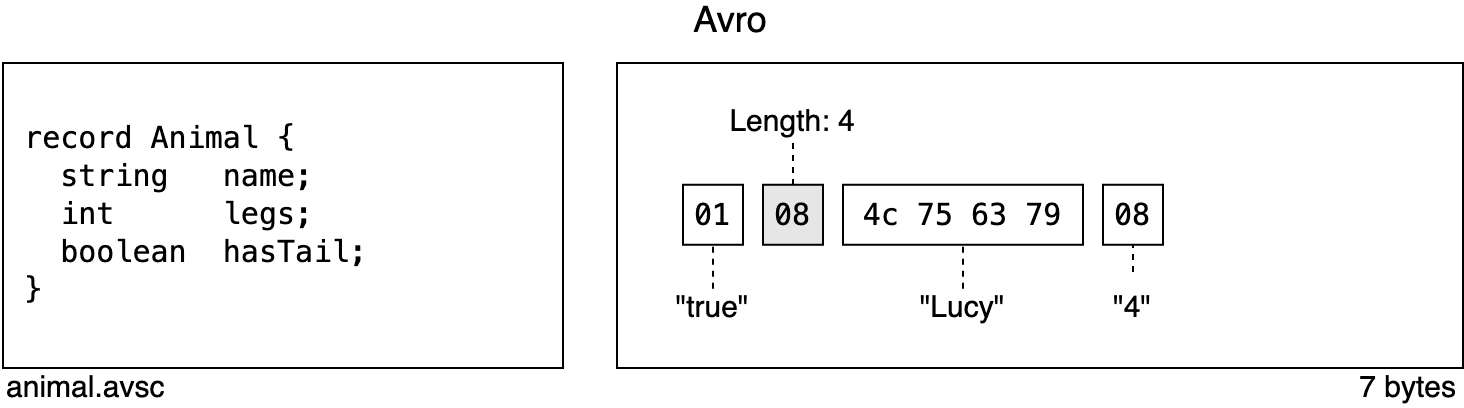
\includegraphics[height=1.5in]{avro}
    \caption{A Avro schema and its associated serialized record }
    \label{fig:avro}
\end{figure}

The deserializer knows which bytes belong to which field by comparing both the reader and writer schemas and by matching fields by their names.

There are other systems that make use of registry's such a Java RMI that uses schema registry's
to perform remote method invocation, the object-oriented equivalent of remote procedure calls, with support for direct
transfer of serialized Java classes and distributed garbage-collection.

\section{Chain of adapters} % (fold)
\label{sec:chain_of_adapters}

The chain of adapters is a design technique for solving the problem of simultaneously deploying
multiple versions of a web service in the face of independently
developed unsupervised clients while maintaining strict backwards compatibility.


\section{Service Integration Adapters} % (fold)
\label{sec:service_integration_adapters}

There has been substantial investigation on the adaptability of services in the context of service-oriented architectures.
Although SOA and microservices are similar in that they both use a separation approach based on services,
these two designs differ in several important ways, most notably in that microservices are loosely coupled whereas SOA services are tightly tied due to common data storage between services.
As a result, adaptability in SOA is focused on service integration and replaceability rather than evolution.

In the setting of SOA, adaptors are used to wrap the various services which are in general heterogeneous,
(communicate with different protocols and support different data formats) so that they can appear as homogeneous and therefore easier to be integrated.

These adaptors presume that data adaptation has already been established by developers at an upper layer,
their primary concern is merging services with different communication protocols and mismatches between operations that have the
same functionality but differ in operation name, number, order or type of operation input/output parameters.

[Developing Adapters for Web Services Integration] presents a taxonomy of all conceivable mismatches as well as remedies to each type in the context of SOA.
Some of the mismatches defined remain important in the context of microservice evolution:
\begin{itemize}
    \item Message Split Mismatch

    This type of differences occurs when the protocol P requires a single message to achieve certain functionality, while in protocol PR the same behavior is achieved by receiving several messages.
    \item Message Merge Mismatch

    This type of differences occurs when protocol P needs to receive several messages for achieving certain
    functionality while protocol PR requires one message to achieve the same functionality.
    \item Differences at the Operation Level

    This type of mismatch occurs when the operation O of S imposes constraints on input parameters,
    which are less restrictive than those of OR input parameters in SR (e.g., differences in value ranges).
\end{itemize}

The two first types of mismatches can be handled in the context of microservice evolution without the use of adaptors.
Essentially, the old endpoints are kept operational but marked as deprecated until there are no more consumers using them, and the new endpoints are provided in parallel.

The latter form of mismatch has an impact on microservice evolution only if service contracts allow refined types.
In other words, when constraints in input parameter are validated in a layer above the application layer.
If validation is conducted in a lower layer, the mismatch can be easily resolved by modifying the application's implementation while keeping the service contract untouched.
